\label{s:hz}
\subsection{Potentially Rocky Planets in the Habitable Zone}
In order for this catalog to be used to understand the occurrence of rocky exoplanets in the habitable zone of a sun-like stars, it needs to identify small, temperate candidates around G-dwarf stars.  In this section we highlight those candidates in that part of the DR25 KOI catalog and mention some of the issues related to using this catalog to calculate occurrence rates.

The DR25 catalog uses the transit depth and the period, along with the DR25 stellar table \citet{Mathur2017ApJS}, to derive the planet radius and the semi-major axis of the planet's orbit.  From these we calculate the insolation flux relative to the insolation flux of the earth:

\begin{equation}
S_{p} = \frac{R_{p}^{2} \cdot (T_{\star}/5777)^{4}}{a^{2}}
\end{equation}

\noindent where $a$ is the semi-major axis of the planet's orbit in AU, \tstar{} is in Kelvin, 5777~K is the effective temperature of the Sun, and \sp{} and \rp{} are in Earth units. The errors for both insolation flux and radii include the errors from the DR25 stellar table. See Figure~\ref{f:hzPlot} for a plot of planet radius against insolation flux at the small, cool end of the DR25 catalog. On this figure the color indicates the stellar temperature and the size of the point indicates the disposition score.  Notice that this part of the catalog is dominated by K and M stars despite the fact that the exoplanet search targets G stars \citet{Batalha2010}.

\begin{figure*}
    \centering
    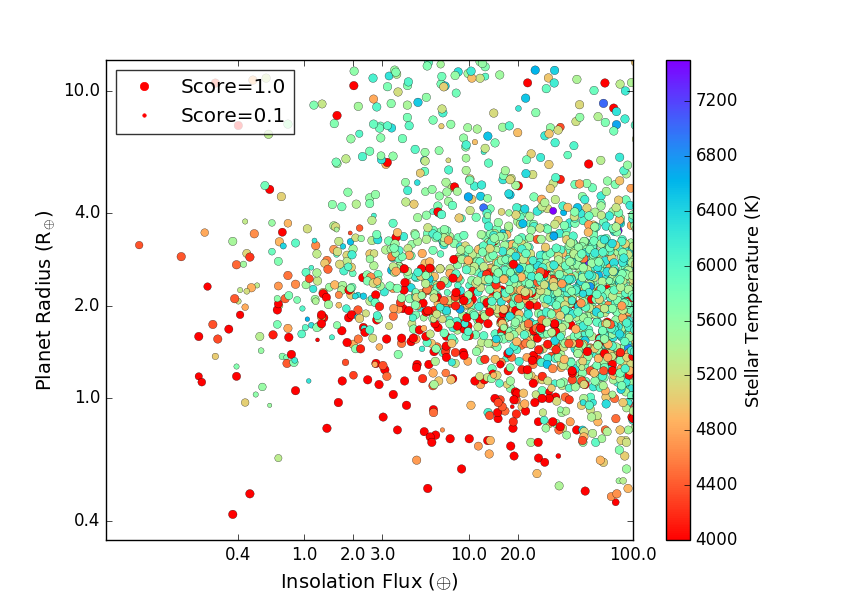
\includegraphics[width=1.1\linewidth]{fig-CatalogRadiusInsolScore.png}
    \caption{DR25 Exoplanet Candidates plotted as planet radius against Insolation Flux, in units of the flux that the Earth receives from the Sun. The stellar temperature is given by the color of the circle and the size of the circle indicates the Disposition Score. The planet radii are derived from the MCMC fits. }
    \label{f:hzPlot}
\end{figure*}

In Table~\ref{t:hz} we highlight the DR25 catalog candidates that are potentially terrestrial and fall in or near the habitable zone of their star.  We select these stars to be any candidate whose one sigma error bars indicate the radius could be smaller than 1.8 \re, and the insolation flux is within the optimistic habitable zone defined by \citet{Kopparapu2013} (i.e. the inner edge is the runaway greenhouse for Venus and the outer edge is given by early Mars [NEED A BETTER DESCRIPTION]). This produces 46 candidates in the DR25 catalog. Of these, 10 are new to the DR25 catalog. In Figure~\ref{f:hzNarrow} we plot those whose score lies above 0.5 because these are the ones with the highest measured reliability.  A manual review of these high score  candidates indicate they all are low signal-to-noise but there is no obvious reason to dismiss the signal.  The reliability measurements for this catalog indicate that for long period, low MES objects (which applies to all those on this plot found on a star with a temperature above 5000\,K) and a disposition score cut greater than 0.5, the reliability is $\approx$80XX per cent, see \S\ref{s:reliability}. 



\begin{figure}
    \centering
    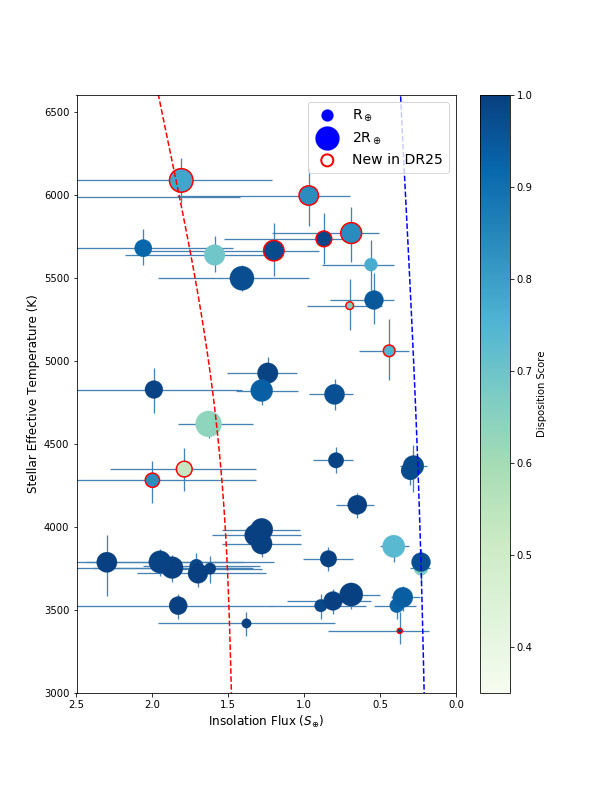
\includegraphics[width=1.1\linewidth]{fig-hzTstarInsol.png}
    \caption{DR25 Exoplanet Candidates plotted as stellar effective temperature against insolation flux. The size of the exoplanet is indicated by the size of the ring, the smaller ring indicates the lower 1sigma bound on the radius and the outer ring is the upper 1 sigma bound.  The color indicate the disposition score with dark green being a score of 1 and white indicating a score of 0.5. Only objects whose error bars indicate that they could be in the habitable zone and whose radii (once considering the error bars) are less than 1.8\re are shown. }
    \label{f:hzNarrow}
\end{figure}


\clearpage
\LongTables
\begin{deluxetable*}{rrrrrlr|lrrlr}
\tablecolumns{12}
\tabletypesize{\scriptsize}
\tablewidth{\linewidth}
\tablecaption{Habitable Zone Planet Candidates}
\tablehead{
\colhead{} & \colhead{} & \colhead{} & \multicolumn{4}{c}{CatalogValues} & \colhead{} & \multicolumn{4}{c}{Confirmed Values} \\ 
\\ 
\colhead{KOI} &
\colhead{SNR} &
\colhead{Score} &
\colhead{\rp} &
\colhead{$F_{\rm p}$} &
\colhead{\tstar} &
\colhead{\rstar} &
\colhead{Confirmed} &
\colhead{\rp} &
\colhead{$S_{\rm p}$} &
\colhead{\tstar} &
\colhead{\rstar} \\ 
\colhead{} &
\colhead{} &
\colhead{} &
\colhead{[\re]} &
\colhead{[$S_{\rm \oplus}$]} &
\colhead{[K]} &
\colhead{[\rsun]} &
\colhead{Name} &
\colhead{[\re]} &
\colhead{[$S_{\rm \oplus}$]} &
\colhead{[K]} &
\colhead{[\rsun]} 
}
\startdata
172.02 & 18.0 & 0.7 & 1.7$^{+0.21}_{-0.22}$ & 1.6$^{+0.59}_{-0.45}$ & 5637$^{+113}_{-101}$ & 0.9$^{+0.1}_{-0.1}$ & Kepler-69 c & 1.7$^{+0.33}_{-0.23}$ & 1.9$^{+0.81}_{-0.57}$ & 5638$^{+168}_{-168}$ & 0.9$^{+0.2}_{-0.1}$  \\ 
238.03 & 11.9 & 0.8 & 2.0$^{+0.33}_{-0.29}$ & 1.8$^{+0.87}_{-0.60}$ & 6086$^{+133}_{-133}$ & 1.2$^{+0.2}_{-0.2}$ & \nodata & \nodata & \nodata & \nodata & \nodata  \\ 
438.02 & 30.6 & 1.0 & 1.9$^{+0.11}_{-0.12}$ & 1.3$^{+0.26}_{-0.25}$ & 3984$^{+71}_{-86}$ & 0.5$^{+0.0}_{-0.0}$ & Kepler-155 c & 1.9$^{+0.11}_{-0.12}$ & 1.3$^{+0.26}_{-0.25}$ & 3984$^{+71}_{-86}$ & 0.5$^{+0.0}_{-0.0}$  \\ 
463.01 & 78.0 & 0.0 & 1.6$^{+0.32}_{-0.29}$ & 1.2$^{+0.72}_{-0.47}$ & 3395$^{+74}_{-67}$ & 0.3$^{+0.1}_{-0.1}$ & Kepler-560 b & 1.6$^{+0.32}_{-0.29}$ & 1.2$^{+0.72}_{-0.47}$ & 3395$^{+74}_{-67}$ & 0.3$^{+0.1}_{-0.1}$  \\ 
494.01 & 35.9 & 1.0 & 1.7$^{+0.21}_{-0.33}$ & 2.3$^{+1.17}_{-1.10}$ & 3787$^{+163}_{-204}$ & 0.5$^{+0.1}_{-0.1}$ & Kepler-577 b & 1.7$^{+0.21}_{-0.33}$ & 2.3$^{+1.17}_{-1.10}$ & 3787$^{+163}_{-204}$ & 0.5$^{+0.1}_{-0.1}$  \\ 
571.05 & 7.7 & 0.7 & 1.2$^{+0.11}_{-0.14}$ & 0.2$^{+0.07}_{-0.06}$ & 3751$^{+75}_{-84}$ & 0.4$^{+0.0}_{-0.1}$ & Kepler-186 f & 1.1$^{+0.08}_{-0.08}$ & 0.3$^{+0.06}_{-0.04}$ & 3755$^{+90}_{-90}$ & 0.5$^{+0.0}_{-0.0}$  \\ 
701.03 & 35.9 & 1.0 & 1.7$^{+0.10}_{-0.07}$ & 1.2$^{+0.27}_{-0.19}$ & 4926$^{+98}_{-98}$ & 0.7$^{+0.0}_{-0.0}$ & Kepler-62 e & 1.6$^{+0.04}_{-0.04}$ & 1.2$^{+0.10}_{-0.10}$ & 4925$^{+70}_{-70}$ & 0.6$^{+0.0}_{-0.0}$  \\ 
812.03 & 18.0 & 1.0 & 1.8$^{+0.12}_{-0.15}$ & 1.3$^{+0.29}_{-0.30}$ & 3950$^{+70}_{-86}$ & 0.5$^{+0.0}_{-0.0}$ & Kepler-235 e & 1.8$^{+0.12}_{-0.15}$ & 1.3$^{+0.29}_{-0.30}$ & 3950$^{+70}_{-86}$ & 0.5$^{+0.0}_{-0.0}$  \\ 
854.01 & 19.3 & 1.0 & 1.9$^{+0.12}_{-0.22}$ & 0.7$^{+0.15}_{-0.19}$ & 3593$^{+71}_{-86}$ & 0.5$^{+0.0}_{-0.1}$ & Kepler-705 b & 1.9$^{+0.12}_{-0.22}$ & 0.7$^{+0.15}_{-0.19}$ & 3593$^{+71}_{-86}$ & 0.5$^{+0.0}_{-0.1}$  \\ 
947.01 & 45.7 & 1.0 & 1.8$^{+0.16}_{-0.21}$ & 1.9$^{+0.52}_{-0.53}$ & 3755$^{+75}_{-84}$ & 0.5$^{+0.0}_{-0.1}$ & Kepler-737 b & 1.8$^{+0.16}_{-0.21}$ & 1.9$^{+0.52}_{-0.53}$ & 3755$^{+75}_{-84}$ & 0.5$^{+0.0}_{-0.1}$  \\ 
1078.03 & 22.2 & 1.0 & 1.9$^{+0.14}_{-0.22}$ & 1.9$^{+0.49}_{-0.55}$ & 3789$^{+75}_{-82}$ & 0.5$^{+0.0}_{-0.1}$ & Kepler-267 d & 1.9$^{+0.14}_{-0.22}$ & 1.9$^{+0.49}_{-0.55}$ & 3789$^{+75}_{-82}$ & 0.5$^{+0.0}_{-0.1}$  \\ 
1404.02 & 10.1 & 1.0 & 0.9$^{+0.16}_{-0.21}$ & 3.0$^{+2.29}_{-1.67}$ & 3751$^{+219}_{-219}$ & 0.5$^{+0.1}_{-0.1}$ & \nodata & \nodata & \nodata & \nodata & \nodata  \\ 
1422.04 & 9.1 & 0.9 & 1.2$^{+0.15}_{-0.18}$ & 0.4$^{+0.15}_{-0.13}$ & 3526$^{+71}_{-78}$ & 0.4$^{+0.0}_{-0.1}$ & Kepler-296 f & 1.8$^{+0.31}_{-0.30}$ & 0.6$^{+0.21}_{-0.25}$ & 3740$^{+130}_{-130}$ & 0.5$^{+0.1}_{-0.1}$  \\ 
1422.05 & 10.5 & 1.0 & 1.1$^{+0.13}_{-0.16}$ & 0.9$^{+0.33}_{-0.30}$ & 3526$^{+71}_{-78}$ & 0.4$^{+0.0}_{-0.1}$ & Kepler-296 e & 1.5$^{+0.26}_{-0.24}$ & 1.4$^{+0.47}_{-0.58}$ & 3740$^{+130}_{-130}$ & 0.5$^{+0.1}_{-0.1}$  \\ 
1596.02 & 16.5 & 0.7 & 1.9$^{+0.13}_{-0.17}$ & 0.4$^{+0.09}_{-0.10}$ & 3883$^{+69}_{-93}$ & 0.5$^{+0.0}_{-0.0}$ & Kepler-309 c & 1.9$^{+0.13}_{-0.17}$ & 0.4$^{+0.09}_{-0.10}$ & 3883$^{+69}_{-93}$ & 0.5$^{+0.0}_{-0.0}$  \\ 
2162.02 & 11.1 & 0.9 & 1.4$^{+0.18}_{-0.18}$ & 2.1$^{+0.76}_{-0.59}$ & 5678$^{+113}_{-102}$ & 0.9$^{+0.1}_{-0.1}$ & \nodata & \nodata & \nodata & \nodata & \nodata  \\ 
2194.03 & 7.9 & 0.5 & 1.4$^{+0.18}_{-0.18}$ & 0.7$^{+0.29}_{-0.22}$ & 5670$^{+113}_{-102}$ & 0.9$^{+0.1}_{-0.1}$ & \nodata & \nodata & \nodata & \nodata & \nodata  \\ 
2418.01 & 11.7 & 0.9 & 1.7$^{+0.12}_{-0.21}$ & 0.3$^{+0.08}_{-0.11}$ & 3576$^{+71}_{-85}$ & 0.5$^{+0.0}_{-0.1}$ & Kepler-1229 b & 1.7$^{+0.12}_{-0.21}$ & 0.3$^{+0.08}_{-0.11}$ & 3576$^{+71}_{-85}$ & 0.5$^{+0.0}_{-0.1}$  \\ 
2626.01 & 14.6 & 1.0 & 1.6$^{+0.20}_{-0.21}$ & 0.8$^{+0.30}_{-0.25}$ & 3554$^{+71}_{-80}$ & 0.4$^{+0.0}_{-0.1}$ & \nodata & \nodata & \nodata & \nodata & \nodata  \\ 
2650.01 & 10.1 & 1.0 & 1.1$^{+0.07}_{-0.10}$ & 1.7$^{+0.35}_{-0.42}$ & 3765$^{+75}_{-83}$ & 0.5$^{+0.0}_{-0.0}$ & Kepler-395 c & 1.1$^{+0.07}_{-0.10}$ & 1.7$^{+0.35}_{-0.42}$ & 3765$^{+75}_{-83}$ & 0.5$^{+0.0}_{-0.0}$  \\ 
2719.02 & 10.0 & 1.0 & 1.5$^{+0.10}_{-0.16}$ & 2.0$^{+0.53}_{-0.58}$ & 4827$^{+129}_{-144}$ & 0.8$^{+0.1}_{-0.1}$ & \nodata & \nodata & \nodata & \nodata & \nodata  \\ 
3010.01 & 12.7 & 1.0 & 1.4$^{+0.07}_{-0.10}$ & 0.8$^{+0.17}_{-0.16}$ & 3808$^{+69}_{-76}$ & 0.5$^{+0.0}_{-0.0}$ & Kepler-1410 b & 1.4$^{+0.07}_{-0.10}$ & 0.8$^{+0.17}_{-0.16}$ & 3808$^{+69}_{-76}$ & 0.5$^{+0.0}_{-0.0}$  \\ 
3034.01 & 11.9 & 1.0 & 1.7$^{+0.12}_{-0.17}$ & 1.7$^{+0.40}_{-0.45}$ & 3720$^{+73}_{-81}$ & 0.5$^{+0.0}_{-0.1}$ & \nodata & \nodata & \nodata & \nodata & \nodata  \\ 
3282.01 & 14.7 & 1.0 & 1.8$^{+0.09}_{-0.13}$ & 1.3$^{+0.26}_{-0.26}$ & 3899$^{+78}_{-78}$ & 0.5$^{+0.0}_{-0.0}$ & Kepler-1455 b & 1.8$^{+0.09}_{-0.13}$ & 1.3$^{+0.26}_{-0.26}$ & 3899$^{+78}_{-78}$ & 0.5$^{+0.0}_{-0.0}$  \\ 
3284.01 & 11.9 & 1.0 & 1.0$^{+0.06}_{-0.07}$ & 1.6$^{+0.37}_{-0.34}$ & 3749$^{+75}_{-84}$ & 0.5$^{+0.0}_{-0.0}$ & Kepler-438 b & 1.1$^{+0.11}_{-0.22}$ & 1.7$^{+0.43}_{-0.50}$ & 3748$^{+112}_{-112}$ & 0.5$^{+0.0}_{-0.1}$  \\ 
3497.01 & 19.6 & 1.0 & 0.8$^{+0.12}_{-0.16}$ & 1.4$^{+0.58}_{-0.58}$ & 3419$^{+67}_{-76}$ & 0.3$^{+0.1}_{-0.1}$ & Kepler-1512 b & 0.8$^{+0.12}_{-0.16}$ & 1.4$^{+0.58}_{-0.58}$ & 3419$^{+67}_{-76}$ & 0.3$^{+0.1}_{-0.1}$  \\ 
4005.01 & 17.8 & 1.0 & 2.2$^{+0.22}_{-0.16}$ & 1.7$^{+0.47}_{-0.31}$ & 5431$^{+81}_{-81}$ & 0.9$^{+0.1}_{-0.1}$ & Kepler-439 b & 2.2$^{+0.11}_{-0.44}$ & 1.9$^{+0.46}_{-0.26}$ & 5431$^{+100}_{-100}$ & 0.9$^{+0.1}_{-0.0}$  \\ 
4036.01 & 14.8 & 1.0 & 1.7$^{+0.10}_{-0.06}$ & 0.8$^{+0.17}_{-0.12}$ & 4798$^{+95}_{-95}$ & 0.7$^{+0.0}_{-0.0}$ & Kepler-1544 b & 1.7$^{+0.10}_{-0.06}$ & 0.8$^{+0.17}_{-0.12}$ & 4798$^{+95}_{-95}$ & 0.7$^{+0.0}_{-0.0}$  \\ 
4087.01 & 15.7 & 1.0 & 1.6$^{+0.10}_{-0.08}$ & 0.7$^{+0.14}_{-0.11}$ & 4133$^{+74}_{-82}$ & 0.6$^{+0.0}_{-0.0}$ & Kepler-440 b & 1.9$^{+0.22}_{-0.22}$ & 1.4$^{+0.32}_{-0.35}$ & 4134$^{+154}_{-154}$ & 0.6$^{+0.0}_{-0.1}$  \\ 
4356.01 & 11.0 & 1.0 & 1.7$^{+0.14}_{-0.20}$ & 0.3$^{+0.09}_{-0.09}$ & 4367$^{+124}_{-155}$ & 0.5$^{+0.0}_{-0.1}$ & Kepler-1593 b & 1.7$^{+0.14}_{-0.20}$ & 0.3$^{+0.09}_{-0.09}$ & 4367$^{+124}_{-155}$ & 0.5$^{+0.0}_{-0.1}$  \\ 
4427.01 & 10.8 & 1.0 & 1.6$^{+0.12}_{-0.14}$ & 0.2$^{+0.06}_{-0.05}$ & 3788$^{+76}_{-84}$ & 0.5$^{+0.0}_{-0.0}$ & \nodata & \nodata & \nodata & \nodata & \nodata  \\ 
4460.01 & 10.7 & 1.0 & 2.0$^{+0.30}_{-0.29}$ & 1.4$^{+0.55}_{-0.44}$ & 5497$^{+82}_{-74}$ & 1.1$^{+0.2}_{-0.2}$ & \nodata & \nodata & \nodata & \nodata & \nodata  \\ 
4550.01 & 9.6 & 0.9 & 1.8$^{+0.05}_{-0.12}$ & 1.3$^{+0.17}_{-0.24}$ & 4821$^{+76}_{-86}$ & 0.8$^{+0.0}_{-0.1}$ & \nodata & \nodata & \nodata & \nodata & \nodata  \\ 
4622.01 & 9.7 & 1.0 & 1.6$^{+0.09}_{-0.06}$ & 0.3$^{+0.06}_{-0.05}$ & 4339$^{+78}_{-87}$ & 0.6$^{+0.0}_{-0.0}$ & Kepler-441 b & 1.6$^{+0.22}_{-0.22}$ & 0.2$^{+0.08}_{-0.06}$ & 4340$^{+177}_{-177}$ & 0.6$^{+0.0}_{-0.1}$  \\ 
4742.01 & 12.9 & 1.0 & 1.3$^{+0.07}_{-0.05}$ & 0.8$^{+0.15}_{-0.11}$ & 4401$^{+78}_{-78}$ & 0.6$^{+0.0}_{-0.0}$ & Kepler-442 b & 1.3$^{+0.11}_{-0.22}$ & 0.7$^{+0.20}_{-0.10}$ & 4402$^{+100}_{-100}$ & 0.6$^{+0.0}_{-0.0}$  \\ 
5375.01 & 7.2 & 0.2 & 5.9$^{+3.64}_{-4.46}$ & 7.5$^{+14.00}_{-7.13}$ & 5142$^{+120}_{-180}$ & 2.8$^{+1.7}_{-2.1}$ & \nodata & \nodata & \nodata & \nodata & \nodata  \\ 
7016.01 & 7.6 & 0.8 & 1.1$^{+0.20}_{-0.10}$ & 0.6$^{+0.32}_{-0.15}$ & 5579$^{+150}_{-150}$ & 0.8$^{+0.1}_{-0.1}$ & Kepler-452 b & 1.6$^{+0.23}_{-0.20}$ & 1.1$^{+0.31}_{-0.19}$ & 5757$^{+85}_{-85}$ & 1.1$^{+0.1}_{-0.1}$  \\ 
7223.01 & 10.3 & 0.9 & 1.6$^{+0.27}_{-0.12}$ & 0.5$^{+0.29}_{-0.13}$ & 5366$^{+160}_{-144}$ & 0.7$^{+0.1}_{-0.1}$ & \nodata & \nodata & \nodata & \nodata & \nodata  \\ 
7703.01 & 7.4 & 0.3 & 2.0$^{+0.61}_{-0.22}$ & 1.0$^{+0.92}_{-0.30}$ & 6031$^{+180}_{-198}$ & 1.0$^{+0.3}_{-0.1}$ & \nodata & \nodata & \nodata & \nodata & \nodata  \\ 
7706.01 & 7.5 & 0.8 & 1.2$^{+0.08}_{-0.16}$ & 2.0$^{+0.55}_{-0.68}$ & 4281$^{+115}_{-140}$ & 0.5$^{+0.0}_{-0.1}$ & \nodata & \nodata & \nodata & \nodata & \nodata  \\ 
7711.01 & 8.5 & 1.0 & 1.3$^{+0.34}_{-0.12}$ & 0.9$^{+0.66}_{-0.22}$ & 5734$^{+154}_{-154}$ & 0.8$^{+0.2}_{-0.1}$ & \nodata & \nodata & \nodata & \nodata & \nodata  \\ 
7716.01 & 7.1 & 0.2 & 1.3$^{+0.25}_{-0.10}$ & 0.4$^{+0.24}_{-0.09}$ & 5700$^{+171}_{-153}$ & 0.7$^{+0.1}_{-0.1}$ & \nodata & \nodata & \nodata & \nodata & \nodata  \\ 
7880.01 & 7.2 & 0.1 & 1.8$^{+0.48}_{-0.26}$ & 1.1$^{+0.80}_{-0.37}$ & 6626$^{+158}_{-217}$ & 1.1$^{+0.3}_{-0.2}$ & \nodata & \nodata & \nodata & \nodata & \nodata  \\ 
7882.01 & 7.2 & 0.5 & 1.3$^{+0.08}_{-0.12}$ & 1.8$^{+0.49}_{-0.47}$ & 4348$^{+130}_{-130}$ & 0.6$^{+0.0}_{-0.1}$ & \nodata & \nodata & \nodata & \nodata & \nodata  \\ 
7894.01 & 8.5 & 0.8 & 1.6$^{+0.49}_{-0.15}$ & 1.0$^{+0.87}_{-0.27}$ & 5995$^{+163}_{-181}$ & 0.9$^{+0.3}_{-0.1}$ & \nodata & \nodata & \nodata & \nodata & \nodata  \\ 
7915.01 & 7.2 & 0.3 & 2.1$^{+0.65}_{-0.43}$ & 2.0$^{+1.81}_{-0.91}$ & 6337$^{+176}_{-220}$ & 1.2$^{+0.4}_{-0.2}$ & \nodata & \nodata & \nodata & \nodata & \nodata  \\ 
7923.01 & 10.0 & 0.8 & 1.0$^{+0.12}_{-0.10}$ & 0.4$^{+0.20}_{-0.13}$ & 5060$^{+192}_{-174}$ & 0.9$^{+0.1}_{-0.1}$ & \nodata & \nodata & \nodata & \nodata & \nodata  \\ 
7930.01 & 8.0 & 0.5 & 1.4$^{+0.11}_{-0.11}$ & 0.3$^{+0.08}_{-0.07}$ & 5031$^{+135}_{-150}$ & 0.6$^{+0.0}_{-0.0}$ & \nodata & \nodata & \nodata & \nodata & \nodata  \\ 
7931.01 & 7.5 & 0.5 & 2.1$^{+0.64}_{-0.35}$ & 2.6$^{+2.40}_{-1.01}$ & 6086$^{+193}_{-214}$ & 1.1$^{+0.3}_{-0.2}$ & \nodata & \nodata & \nodata & \nodata & \nodata  \\ 
7932.01 & 7.2 & 0.2 & 1.0$^{+0.22}_{-0.15}$ & 0.5$^{+0.33}_{-0.18}$ & 5637$^{+169}_{-152}$ & 0.8$^{+0.2}_{-0.1}$ & \nodata & \nodata & \nodata & \nodata & \nodata  \\ 
7938.01 & 7.5 & 0.5 & 2.3$^{+0.53}_{-1.32}$ & 8.6$^{+6.29}_{-7.18}$ & 5989$^{+213}_{-192}$ & 2.5$^{+0.6}_{-1.4}$ & \nodata & \nodata & \nodata & \nodata & \nodata  \\ 
7953.01 & 7.3 & 0.3 & 1.4$^{+0.33}_{-0.12}$ & 0.6$^{+0.37}_{-0.14}$ & 5580$^{+150}_{-166}$ & 0.9$^{+0.2}_{-0.1}$ & \nodata & \nodata & \nodata & \nodata & \nodata  \\ 
7954.01 & 8.9 & 0.8 & 1.7$^{+0.46}_{-0.14}$ & 0.7$^{+0.52}_{-0.18}$ & 5769$^{+155}_{-172}$ & 0.8$^{+0.2}_{-0.1}$ & \nodata & \nodata & \nodata & \nodata & \nodata  \\ 
7992.01 & 8.7 & 0.1 & 1.8$^{+0.56}_{-0.18}$ & 2.1$^{+1.81}_{-0.61}$ & 6461$^{+155}_{-213}$ & 1.0$^{+0.3}_{-0.1}$ & \nodata & \nodata & \nodata & \nodata & \nodata  \\ 
8000.01 & 8.7 & 1.0 & 1.7$^{+0.43}_{-0.14}$ & 1.2$^{+0.90}_{-0.30}$ & 5663$^{+169}_{-152}$ & 0.8$^{+0.2}_{-0.1}$ & \nodata & \nodata & \nodata & \nodata & \nodata  \\ 
8012.01 & 7.7 & 1.0 & 0.4$^{+0.17}_{-0.12}$ & 0.4$^{+0.47}_{-0.19}$ & 3374$^{+112}_{-82}$ & 0.2$^{+0.1}_{-0.1}$ & \nodata & \nodata & \nodata & \nodata & \nodata  \\ 
8048.01 & 7.2 & 0.3 & 1.3$^{+0.36}_{-0.11}$ & 0.9$^{+0.70}_{-0.23}$ & 6156$^{+167}_{-186}$ & 0.8$^{+0.2}_{-0.1}$ & \nodata & \nodata & \nodata & \nodata & \nodata  \\ 
8085.01 & 7.9 & 0.4 & 1.7$^{+0.46}_{-0.31}$ & 1.0$^{+0.82}_{-0.41}$ & 5979$^{+161}_{-179}$ & 1.0$^{+0.3}_{-0.2}$ & \nodata & \nodata & \nodata & \nodata & \nodata  \\ 
8107.01 & 7.6 & 0.4 & 1.7$^{+0.45}_{-0.67}$ & 2.3$^{+1.88}_{-1.60}$ & 6180$^{+195}_{-238}$ & 1.9$^{+0.5}_{-0.8}$ & \nodata & \nodata & \nodata & \nodata & \nodata  \\ 
8174.01 & 7.4 & 0.7 & 0.6$^{+0.07}_{-0.07}$ & 0.7$^{+0.28}_{-0.21}$ & 5332$^{+160}_{-144}$ & 0.8$^{+0.1}_{-0.1}$ & \nodata & \nodata & \nodata & \nodata & \nodata  \\ 
8242.01 & 7.1 & 0.2 & 1.4$^{+0.32}_{-0.11}$ & 0.8$^{+0.56}_{-0.19}$ & 5762$^{+155}_{-155}$ & 0.8$^{+0.2}_{-0.1}$ & \nodata & \nodata & \nodata & \nodata & \nodata  \\ 
8246.01 & 7.2 & 0.2 & 1.6$^{+0.45}_{-0.37}$ & 1.5$^{+1.27}_{-0.71}$ & 6067$^{+182}_{-182}$ & 1.2$^{+0.3}_{-0.3}$ & \nodata & \nodata & \nodata & \nodata & \nodata  \\ 
8253.01 & 7.9 & 0.1 & 0.9$^{+0.13}_{-0.04}$ & 0.6$^{+0.22}_{-0.08}$ & 5547$^{+74}_{-83}$ & 0.9$^{+0.1}_{-0.0}$ & \nodata & \nodata & \nodata & \nodata & \nodata  \\ 
8259.01 & 7.5 & 0.3 & 1.7$^{+0.52}_{-0.18}$ & 1.1$^{+1.00}_{-0.34}$ & 6299$^{+170}_{-226}$ & 0.9$^{+0.3}_{-0.1}$ & \nodata & \nodata & \nodata & \nodata & \nodata  \\ 
8272.01 & 7.6 & 0.1 & 1.1$^{+0.37}_{-0.13}$ & 1.1$^{+1.04}_{-0.32}$ & 6263$^{+169}_{-188}$ & 1.0$^{+0.3}_{-0.1}$ & \nodata & \nodata & \nodata & \nodata & \nodata  \\ 
\enddata
\tablecomments{KOIs with confirmed planet numbers have been confirmed as planetary in nature either via ground-based follow-up observations or statistical analyses. In these cases we list the confirmed \kepler{} planet number, confirmed values for the planet radius, insolation flux, and stellar effective temperature and radius, and reference for the confirmation study.}
\label{t:hz}
\end{deluxetable*}

